%%%%%%%%%%%%%%%%%%%%%%%%%%%%%%%%%%%%%%%%%%%%%%%%%%%%%%%%%%%%%
%%
%%
%%     NPR's  Nature template...  
%%     v1.0.0   Thu Dec  8 19:05:57 EST 2016
%%                                                                         
%%
%%%%%%%%%%%%%%%%%%%%%%%%%%%%%%%%%%%%%%%%%%%%%%%%%%%%%%%%%%%%%
\documentclass{nature}
%\documentclass{natureprintstyle}

\usepackage{graphicx, fancyhdr, subfigure}
\usepackage{epsfig, psfig, epsf}
\usepackage{amsmath, amssymb, cancel, mathptmx}
\usepackage[T1]{fontenc}
\usepackage{dcolumn}  %%  Align table columns on decimal point
\usepackage{bm}           %%  bold math
\usepackage{hyperref,ifthen}
\usepackage{verbatim, threeparttable}
\usepackage[square,sort,comma,numbers]{natbib}

\newcommand{\oiii}{[O\,{\sc iii}]\ }
\newcommand{\nii}{N\,{\sc ii}\ }



\bibliographystyle{naturemag}

\title{A new interpretation of optical and infrared variability in quasars}

\author{Nicholas~P.~Ross$^{1}$ et al.  
%K. E. Saavik Ford$^{2,3,4}$
%Matthew Graham$^{5}$
%Barry McKernan$^{2,3,4}$
%Daniel Stern, 
%Aaron Meisner, 
%Andrew Drake, 
%Arjun Dey, 
%David Schlegel, 
%Roberto Assef, 
%Jun, 
%Peter Eisenhardt, 
%Djorgovsk
}
%%
% Saavik~K.~Ford,$^{7}$, Barry~L.~McKernan$^{7}$,
% Daniel~Stern$^{3}$, Aaron~Meisner$^{2}$, 
% Matthew~Graham$^{4}$, 
% Arjun~Dey$^{5}$ \& David~J.~Schlegel$^{2}$ 
% Andrew~Drake$^{4}$, 
% Roberto~J.~Assef$^{6},
% Mislav~Balokovic$^{6}, 
% Murray~Brightman$^{4}, 
% for the DECaLS Consortium. 

\begin{document}

\maketitle

\begin{affiliations}
  \item Institute for Astronomy, University of Edinburgh, Royal Observatory, Blackford Hill, Edinburgh EH9 3HJ, United Kingdom 
%  \item Department of Science, BMCC, City University of New York, New York, NY 10007, USA
 % \item Department of Astrophysics, American Museum of Natural History, New York, NY 10024, USA
 % \item  Graduate Center, City University of New York, 365 5th Avenue, New York, NY 10016, USA
%XSXS\item Cahill Center for Astronomy and Astrophysics, California Institute of Technology, Mail Code 249/17, 1200 E California Blvd, Pasadena CA 91125, USA
 % \item Department of Astrophysics is located in the Rose Center for Earth and Space, American Museum of Natural History, Central Park West at 79th Street, New York, NY 10024, U.S.A
  %\item Jet Propulsion Laboratory, California Institute of Technology, 4800 Oak Grove Drive, Mail Stop 169-221, Pasadena, CA 91109, USA 
  %\item California Institute of Technology, 1200 East California Boulevard, Pasadena, CA 91125, USA
  %\item Steward Observatory, 933 North Cherry Avenue, Tucson, AZ 85721, U.S.A.
%  \item Universidad Diego Portales, Av Republica 180, Santiago, Regi ́on Metropolitana, Chile}
%  \item Lawrence Berkeley National Laboratory, 1 Cyclotron Road, Berkeley, CA 92420, U.S.A. 
\end{affiliations}


\begin{abstract}
Changing-look quasars are a recently identified class of active galaxies in 
which the strong UV continuum and/or broad optical hydrogen emission
lines associated with unobscured quasars either appear or disappear on
timescales of months to years \cite{LaMassa2015, Runnoe2016,
MacLeod2016, Ruan2016, Yang2017}.  The physical processes responsible for this
behaviour are still debated, but changes in the black hole accretion
rate or accretion disk structure appear more likely than changes in
obscuration \cite{Hutsemekers2017, Sheng2017}.  Here we report on
three epochs of spectroscopy of SDSS J110057.70-005304.5, a quasar at
a redshift of $z=0.378$ whose UV continuum and broad hydrogen
emission lines have dramatically faded over the past $\approx$20
years. The change in this quasar was initially seen in the infrared,
and an archival spectrum from 2010 shows an intermediate phase of the
transition during which the flux below rest-frame 3400\AA\ has
collapsed. This combination is unique compared to previously published examples of
changing-look quasars, and is best explained by dramatic changes in
the innermost regions of the accretion disk. The optical continuum has
been rising again since mid-2016, leading to a prediction of a rise in
hydrogen emission line flux in the next year. If our model is
confirmed, the physics of changing-look quasars are governed by
processes at the innermost stable circular orbit (ISCO) around the
black hole, and the structure of the innermost disk. The easily
identifiable and monitored changing-look quasars would then provide a
new probe of the strong gravity regime.
\end{abstract}



%%%%%%%%%%%%%%%%%%%%%%%%%%%%%%%%%%%%%%%%%%%%%%%%%%%%%%%%%%%%%
%%%%%%%%%%%%%%%%%%%%%%%%%%%%%%%%%%%%%%%%%%%%%%%%%%%%%%%%%%%%%
%%
%%   SECTION 1  SECTION 1  SECTION 1  SECTION 1  SECTION 1  SECTION 1  
%%   SECTION 1  SECTION 1  SECTION 1  SECTION 1  SECTION 1  SECTION 1  
%%   SECTION 1  SECTION 1  SECTION 1  SECTION 1  SECTION 1  SECTION 1  
%%
%%%%%%%%%%%%%%%%%%%%%%%%%%%%%%%%%%%%%%%%%%%%%%%%%%%%%%%%%%%%%
%%%%%%%%%%%%%%%%%%%%%%%%%%%%%%%%%%%%%%%%%%%%%%%%%%%%%%%%%%%%%
%\section{Introduction}
The changing-look quasar phenomenon, where the dramatic disappearance,
or appearance, of the strong UV continuum and/or the prominent broad
optical emission lines is seen on month-to-year timescales, is now
widely observed \cite{LaMassa2015, MacLeod2016, Runnoe2016, Ruan2016,
Gezari2017, Rumbaugh2017, Yang2017} yet poorly understood. Changes in
obscuration are generally disfavoured due to the timescales currently
observed \cite{Hutsemekers2017, Sheng2017}, and it is clear that
changing-look quasars are a key laboratory for understanding accretion
physics and active galactic nuclei (AGN).

The Shakura-Sunyaev $\alpha-$disk model \cite{SS73} has long been used
to (over-)simply describe the basic properties of optically thick,
geometrically thin accretion disks. Indeed we utilize the alpha-disk
model in this paper, however, the model is ad hoc, only parameterizing
disk viscosity, and does not permit predictions of global changes to
the disk \cite{King2012}. Real AGN disks seem to be cooler \cite[e.g.,
][]{Lawrence2012} and larger \cite[e.g.,][]{Pooley2007, Morgan2010,
Morgan2012, Mosquera2011} than the alpha-disk model predicts, and
viscosity seems likely due to magnetic fields \cite{Balbus_Hawley1991}
with additional contributions to turbulence from the effects of
embedded objects in the disk \cite[e.g., ][]{McKernan2014}.

Changing-look quasars have traditionally been discovered by looking
for large, $| \Delta m | >1$ magnitude changes in optical light curves
of quasars or galaxies (e.g. across 3720\AA\ $< \lambda <$ 5680\AA, in
the $g$-band). However, we have taken advantage of the ongoing
Near-Earth Object WISE Reactivation mission \cite[NEOWISE-R;
][]{Mainzer2014, Meisner2017a, Meisner2017b}, as well as the Dark
Energy Camera Legacy Survey (DECaLS\footnote{{\tt
legacysurvey.org/decamls/}}) in order to discover new changing-look
quasars. While previous efforts have used the 1-year baseline of the
WISE mission to identify CLQs \cite[e.g., []{Assef2017}, our team is
the first to extend .  Our team is the first to extend this selection
to the infrared using NEOWISE-R mission data, and we have identified a
sample of SDSS quasars that show dramatic decreases in their IR flux
over the course of a few years. These changes are on timescales too
short to be due to changes in obscuration, so a different explanation
is needed.

In this article we present the $z=0.378$ quasar SDSS
J110057.70-005304.5 (hereafter J1100-0053) for which we have spectral
observations showing a transition in the blue-continuum slope
traditionally associated with the blackbody spectrum of an object with
broad hydrogen emission lines, into a `dim state' where the rest-frame
UV flux is suppressed, and then returning to a blue-continuum sloped
quasar.  We present a model that invokes changes at the ISCO to be the
triggering event for the change in the accretion disk, which along
with the changes in the broad emission lines, explains a major change
to the disk interior to 150$r_{g}$ (where $r_{\rm g}$ is the
gravitational radius; $r_{\rm g}=\frac{GM}{c^2}$) as well as the IR
light curves. Critically, our model makes predictions to the future
behaviour of J1100-0053.
 
\begin{figure}
  \centering
  %% trim=l b r t 
  % 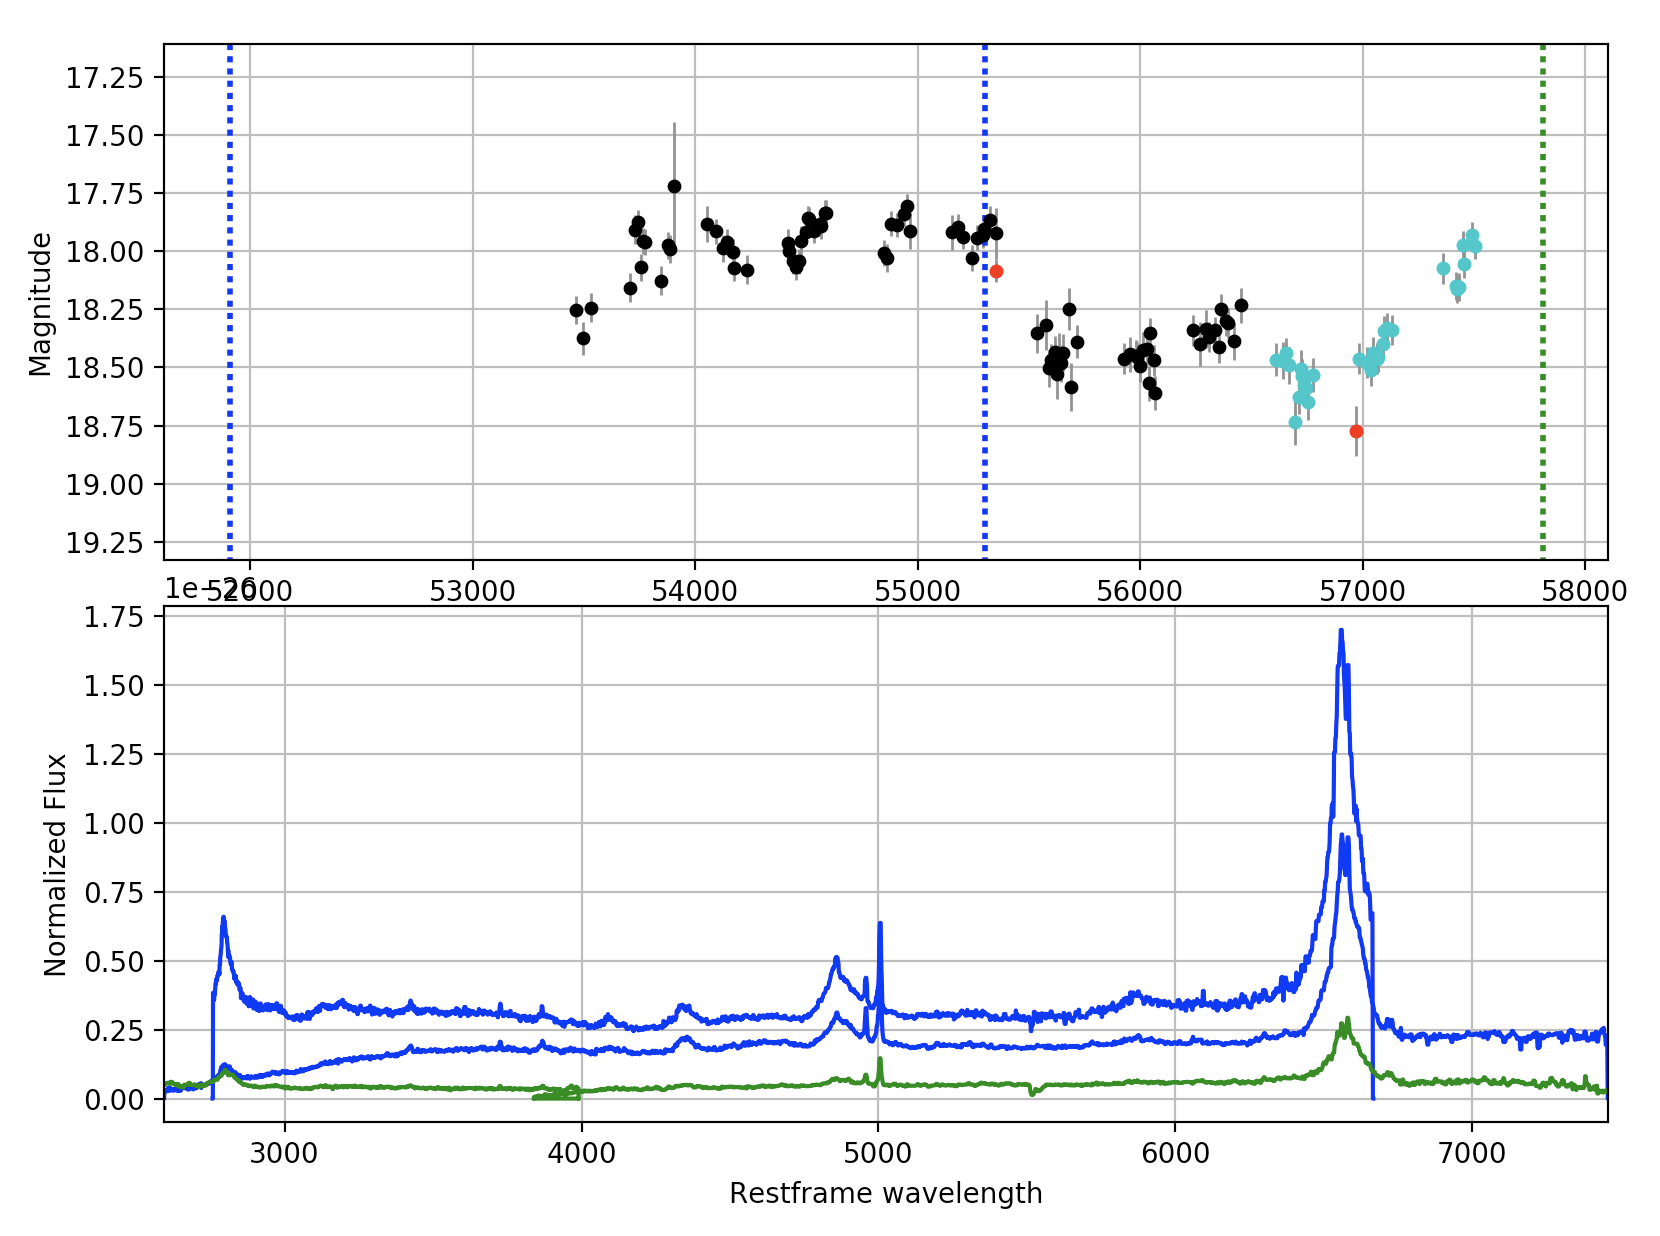
\includegraphics[width=8.00cm, height=7.50cm, trim=0.0cm 0.0cm 0.0cm 0.0cm, clip] {J110057_CRTS_lightcurve_v0pnt1.png}
  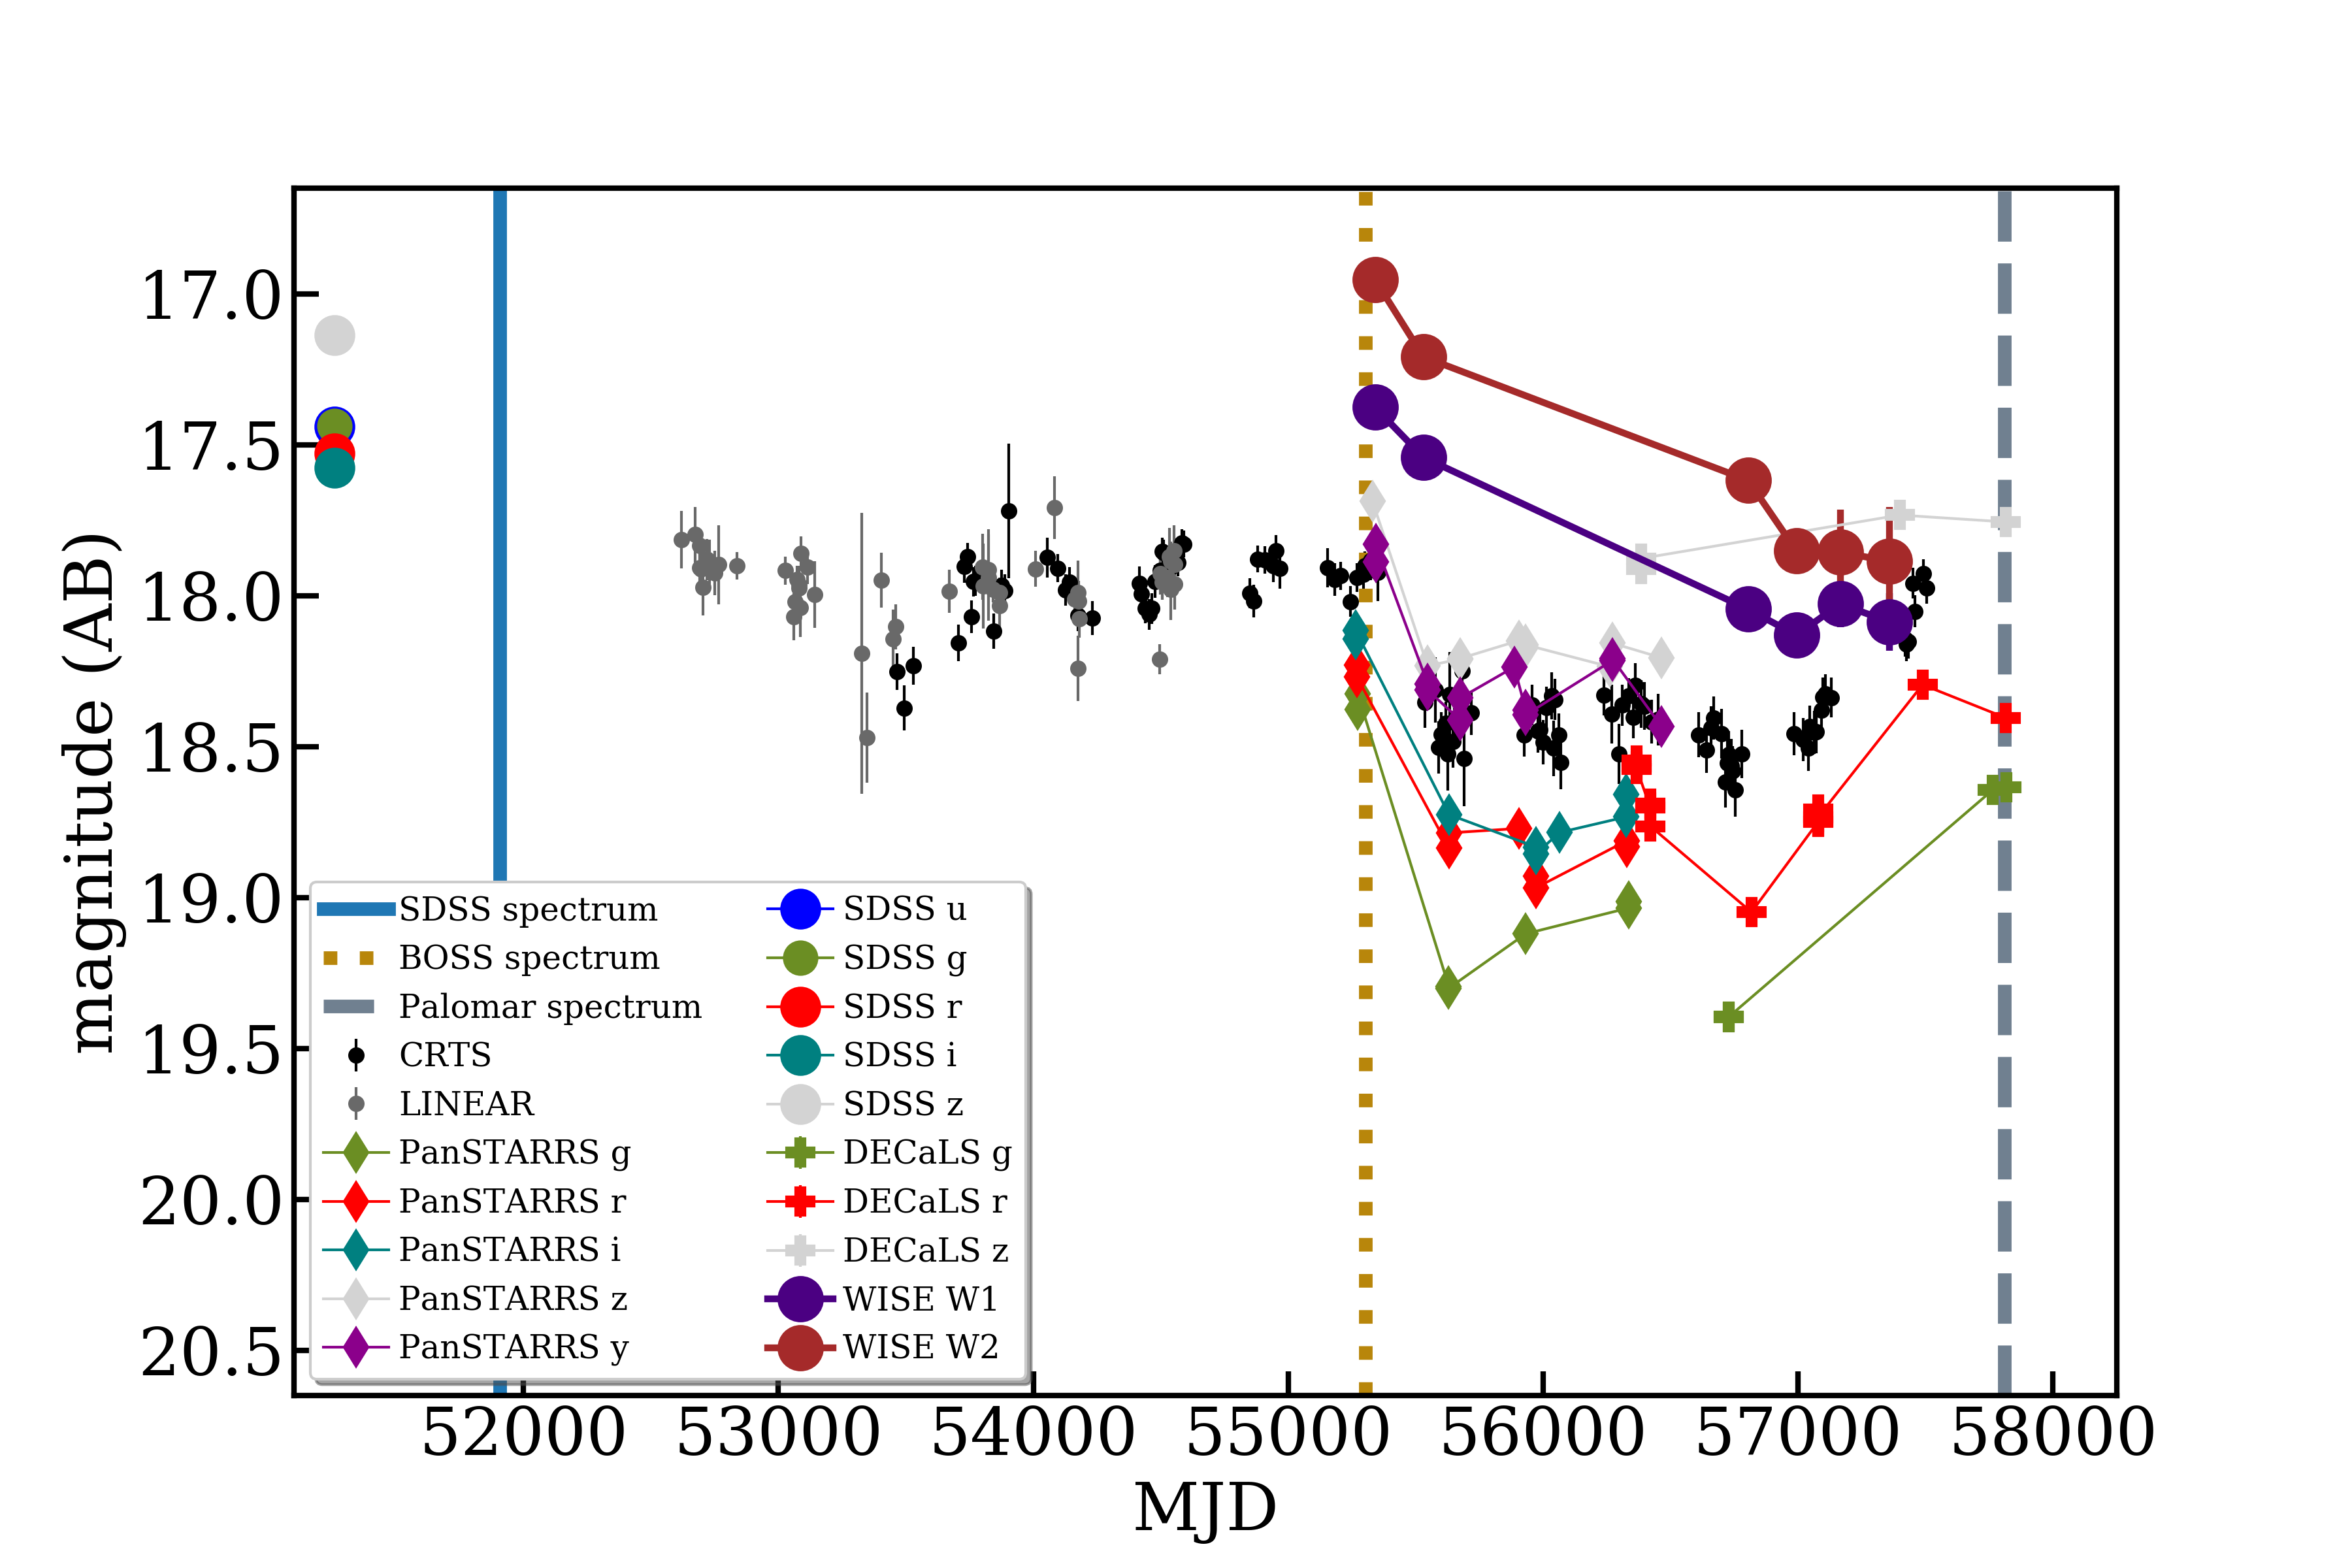
\includegraphics[width=16.00cm, height=10.00cm, trim=0.0cm 0.0cm 0.0cm 0.0cm, clip]
  {../plots/lc/J110057_lc_20171204v1.png}
  \caption[]{
    Multi-wavelength light curve of J1100-0053,
    including optical data from LINEAR, CRTS, SDSS, PanSTARRS and
    DECaLS, and mid-IR data from the WISE satellite.  The three vertical
    lines illustrate the epochs of the three optical spectra presented
    in Figure 2.  J1100-0053 was flagged for further study due to the
    extreme IR fading observed by WISE.  Note that the optical emission
    has been recovering over the past few years; we predict the IR
    emission will similarly recover over the next few years.}
  \label{fig:J110057_LC_CRTS}
\end{figure}


\begin{figure}
  \centering
  %% trim=l b r t 
  \includegraphics[width=17.00cm, height=12.00cm, trim=0.0cm 0.0cm 0.0cm 0.0cm, clip]
  {../plots/spectra/w1100m0052_sdss_wmodels.jpg}
  \caption[]{
    Optical spectra of J1100-0053 obtained on MJD 51908 (blue; SDSS), 55302,
    (red; BOSS) and 57809 (black; Palomar/DBSP).  {\it Left::} The full
    optical spectra; {\it Right (top)::} Zoom in on the H$\beta$-\oiii
    complex; {\it Right (bottom)::} Zoom in on the H$\alpha$-\nii complex.
  }
  \label{fig:J110057_spectra}
\end{figure}
%%%%%%%%%%%%%%%%%%%%%%%%%%%%%%%%%%%%%%%%%%%%%%%%%%%%%%%%%%%%% 
%%%%%%%%%%%%%%%%%%%%%%%%%%%%%%%%%%%%%%%%%%%%%%%%%%%%%%%%%%%%% 
%%
%%   SECTION 2   SECTION 2   SECTION 2   SECTION 2   SECTION 2   SECTION 2  
%%   SECTION 2   SECTION 2   SECTION 2   SECTION 2   SECTION 2   SECTION 2  
%%   SECTION 2   SECTION 2   SECTION 2   SECTION 2   SECTION 2   SECTION 2  
%%
%%%%%%%%%%%%%%%%%%%%%%%%%%%%%%%%%%%%%%%%%%%%%%%%%%%%%%%%%%%%%
%%%%%%%%%%%%%%%%%%%%%%%%%%%%%%%%%%%%%%%%%%%%%%%%%%%%%%%%%%%%%
\section{Target Selection and Observations}  
We started by matching the SDSS-III BOSS Data Release 12 Quasar
catalog \cite[DR12Q; ][]{Paris2017} to the NEOWISE-R IR data (WISE W1
at 3.4$\mu$m, WISE W2 at 4.6$\mu$m). We found $\sim$200 objects
identified by a factor of 2 or more change in the observed WISE W1 and
W2 bands over the course of typically three or four years
\citep[see][and the Supplemental Material for the detailed NEOWISE-R
selection]{Meisner2017b}. Scanning these 200 objects, we also examined
the change in optical colour using the SDSS and DECaLS imaging surveys
in order to identify changes suggestive of changing-look quasars.
From this inspection, a priority list of $\approx70$ quasar targets
was derived and we obtained new optical spectroscopy from the Palomar
5m telescope.  J1100-0053 was one of these 70 objects, but critically,
had spectra from both SDSS and BOSS and was thus a priority target.

Figure~\ref{fig:J110057_LC_CRTS} presents the light curve of
J1100-0053.  Along with WISE IR data, optical data from the SDSS,
Catalina Real-time Transient Survey \citep[CRTS;][]{Drake2009,
Mahabal2011}, LINEAR \citep{Sesar2011} and PanSTARRS
\citep{Kaiser2010, Stubbs2010, Tonry2012, Magnier2013} are available.
Figure~\ref{fig:J110057_spectra} shows the three optical spectra of
J1100-0053 from the SDSS, BOSS and Palomar observations taken on MJD
51908 (UT 2000 December 30), 55302 (UT 2010 April 16) and 57809 (UT
2017 February 25), respectively.  The first-epoch SDSS spectrum shows
a typical blue quasar, but blue continuum then collapses in the second
epoch BOSS spectrum taken 10 years later. However, the blue continuum
has then returned in the third epoch spectrum 7 years later, albeit at
a diminished flux from the initial spectrum.  The Supplemental
Material gives further observation details including an achival ROSAT
detection.


%%%%%%%%%%%%%%%%%%%%%%%%%%%%%%%%%%%%%%%%%%%%%%%%%%%%%%%%%%%%%
%%%%%%%%%%%%%%%%%%%%%%%%%%%%%%%%%%%%%%%%%%%%%%%%%%%%%%%%%%%%%
%%
%%   SECTION 3   SECTION 3   SECTION 3   SECTION 3   SECTION 3   SECTION 3  
%%   SECTION 3   SECTION 3   SECTION 3   SECTION 3   SECTION 3   SECTION 3  
%%   SECTION 3   SECTION 3   SECTION 3   SECTION 3   SECTION 3   SECTION 3  
%%
%%%%%%%%%%%%%%%%%%%%%%%%%%%%%%%%%%%%%%%%%%%%%%%%%%%%%%%%%%%%%
%%%%%%%%%%%%%%%%%%%%%%%%%%%%%%%%%%%%%%%%%%%%%%%%%%%%%%%%%%%%%
\begin{figure*}
  %% trim=l b r t 
  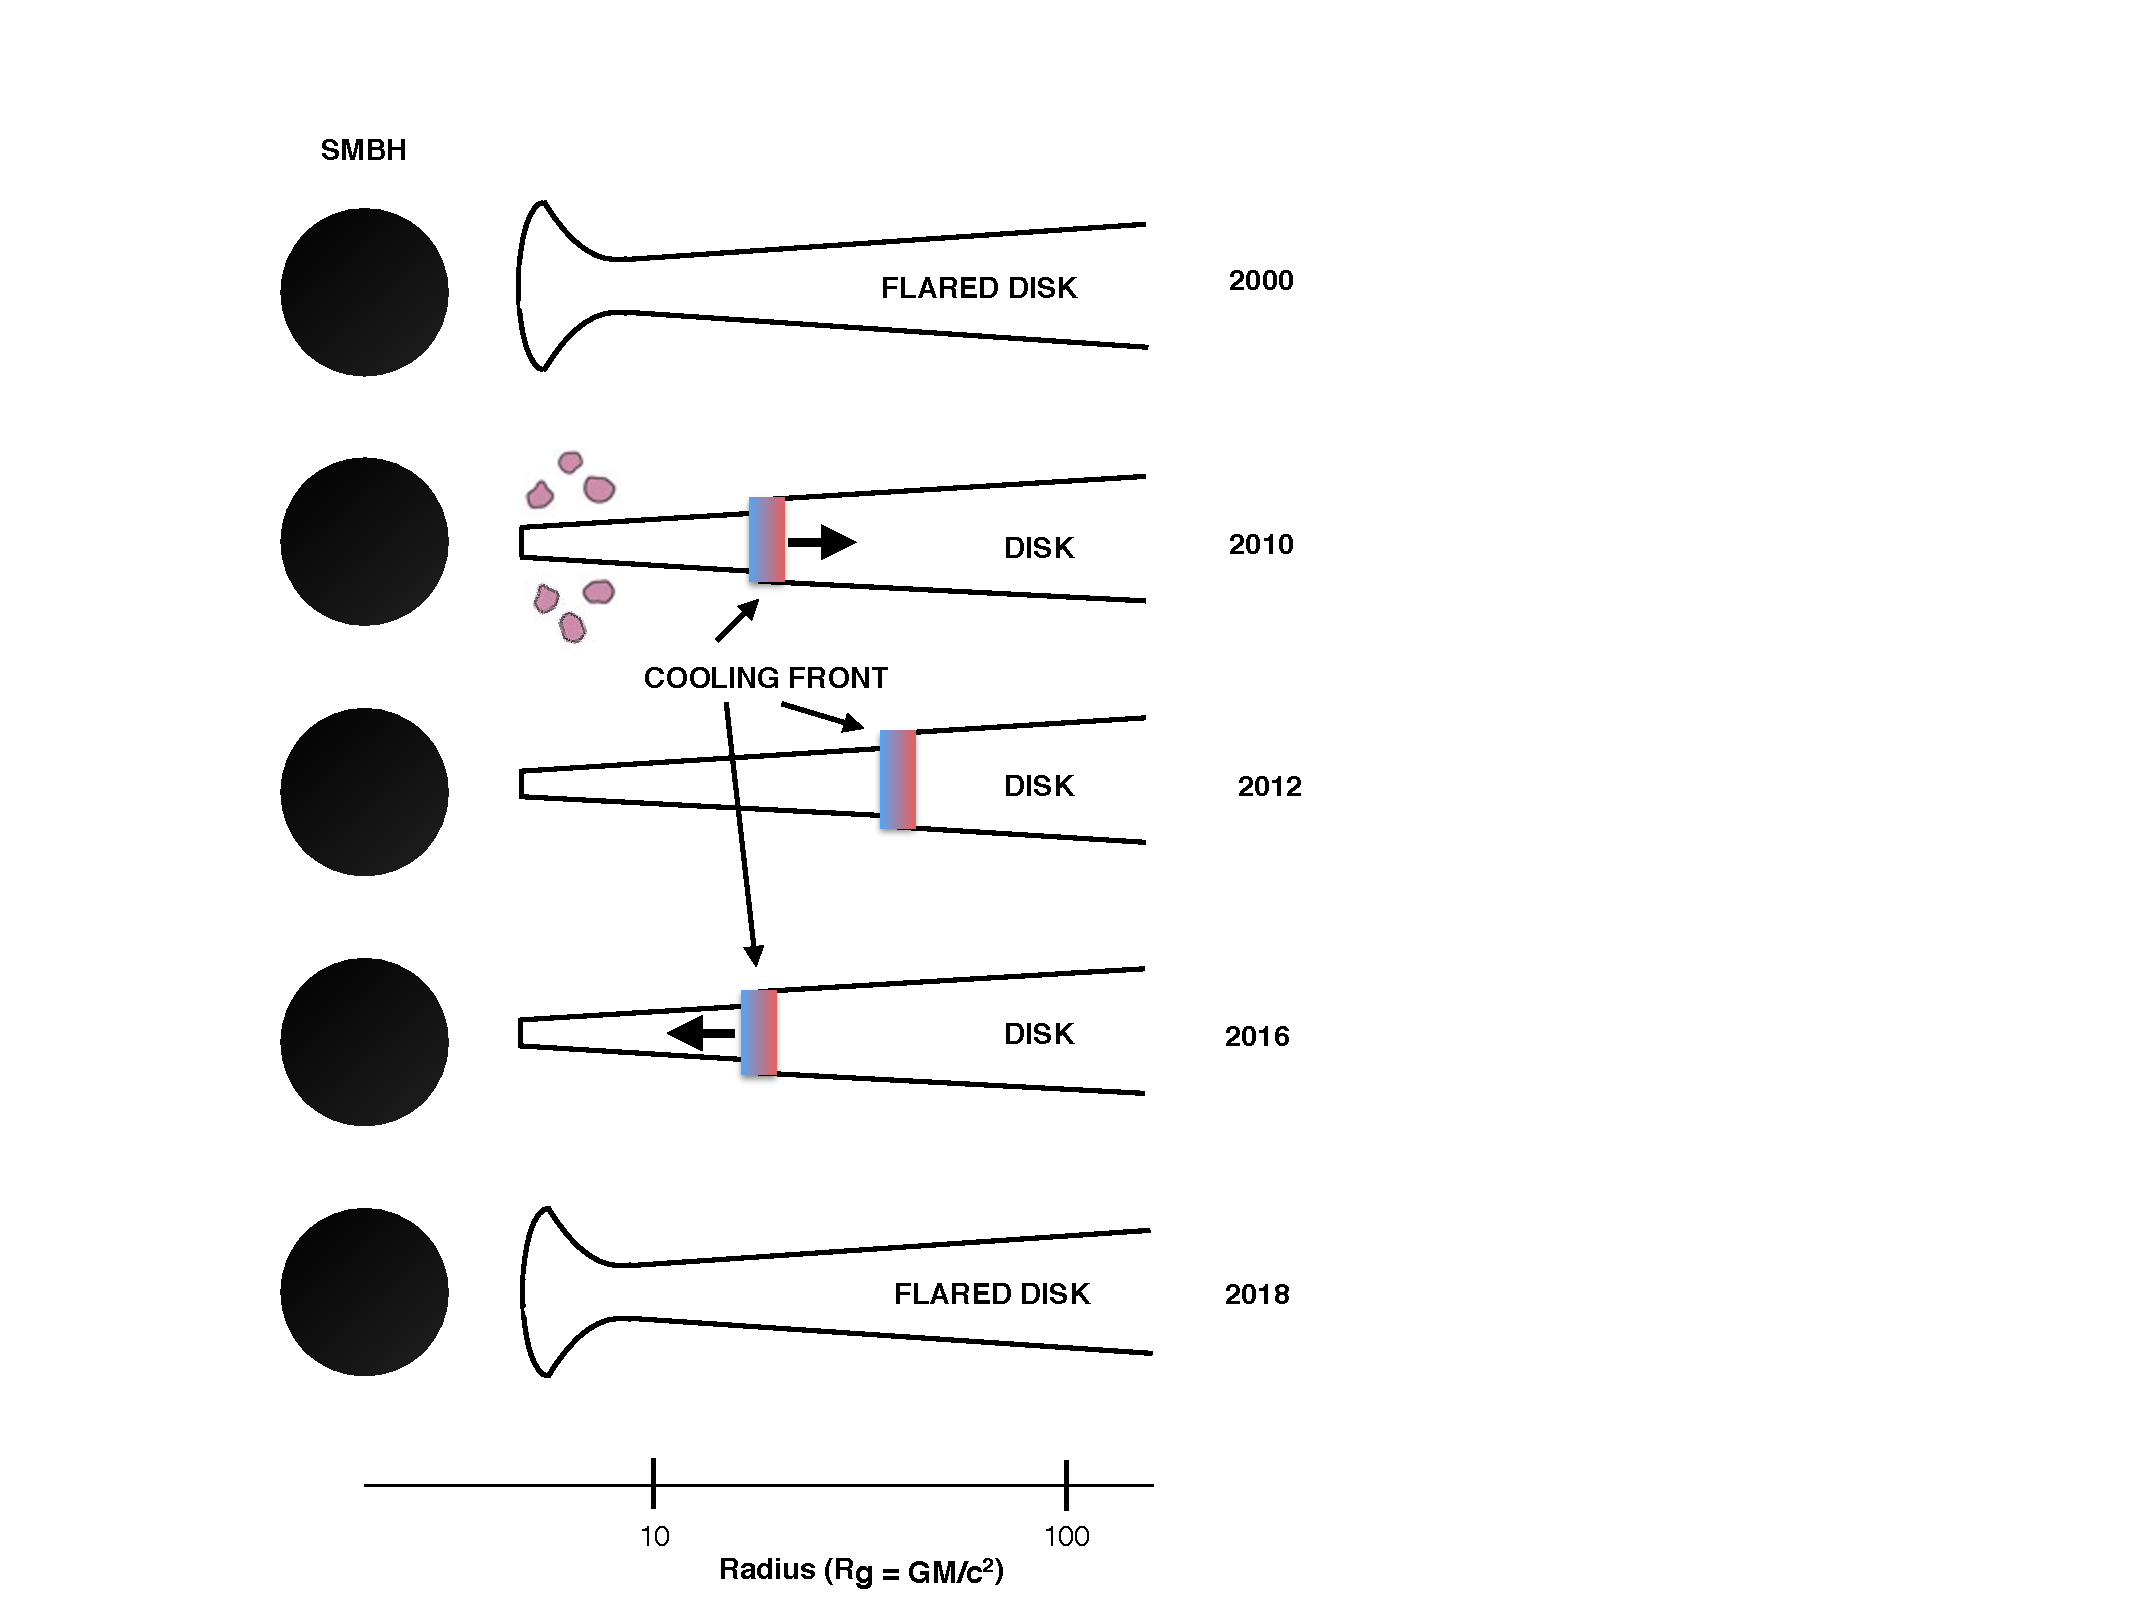
\includegraphics[width=15.4cm, height=18.75cm, trim=0.0cm 0.0cm 0.0cm 0.0cm, clip]
  {../plots/models/cartoon_v2.pdf}
  \centering
  \caption[]{
    A cartoon illustration of our model explaining the unusual spectral
    evolution of J1100-0053. In 2000, corresponding to the SDSS
    spectral epoch, the quasar has a standard modified $\alpha$-disk, with
    a geometrically thin, optically thick disk that is inflated near
    the ISCO, i.e., the inner edge of the accretion disk.  Circa 2007,
    an event occurs that deflates the inner disk, leaving some scattering
    clouds, and causing a cooling front to propogate inwards.  Circa
    2012, the front reflects back, re-heating the inner accretion disk.
    We predict that in the next year, the quasar should roughly return
    to its initial state.}
  \label{fig:J110057_diskmodel}
\end{figure*}
\section{Discussion}   
Our model of thermal emission from a multicolour disk implies 
changes in the region from the ISCO to $\sim$few tens-100 $r_{\rm g}$
are required to suppress flux into the observed
$g$-band. In particular, we suggest a physical collapse of the disk
scale height due to a cooling front propagating outward from the ISCO.

For J1100-0053 we apply our model as follows. We start with an
inflated (slim) disk. We assume a non-zero torque at the ISCO and
$h/r\sim0.2$ inside of $r\sim100 r_{\rm g}$. This is the initial state
circa 2000 (MJD 51900). A non-zero torque at the ISCO implies that
matter in the plunging region is connected (however weakly) to matter
outside the ISCO, probably by magnetic fields \cite[e.g.,
][]{Gammie1999, Agol_Krolik2000}. A non-zero torque at the ISCO
maintains a hotter innermost disk than a condition of zero torque at
the ISCO, and an assumption of non-zero torque is particularly
appropriate if disk viscosity and accretion are indeed driven by
magnetic fields. In order to explain data subsequent to 2007, we
assume a cooling front propagates out from the ISCO over a timescale
$t_{\rm front}$. The simplest explanation is that the non-zero torque
condition at the ISCO changes to a (more nearly) zero-torque
condition, leading to a dramatically cooler, thinner disk near the
ISCO. As the cooling front propagates, the drop in temperature leads
to a drop in flux. Our model requires cooler regions behind the front
to emit 10\% the flux of the initial hotter disk, and the disk height
drops by a factor $\sim$2. The dimming of the inner disk causes a drop
in the ionizing photon flux ($L_{\rm ion}$), which will cause: the
Balmer lines to drop in flux after a light travel time of months and
the IR from the outer disk/torus to drop in flux after a light travel
time of $\sim$3 years.

If the inner accretion disk is usually inflated \cite[see e.g.,
][]{Sirko_Goodman2003, Thompson2005, Hopkins_Quataert2011}, such a
cooling front will naturally produce: 1) a collapse in the scale
height of the disk; 2) a decrease in flux moving from UV to longer
optical wavelengths; 3) a temporarily thicker scattering atmosphere,
further decreasing flux at short wavelengths.  This model implies
changes to the optical emission moving from shorter to longer
wavelengths (as the radius of the cooling front increases), on
months-to-years-long timescales. It also predicts a longer time to
recover the original flux (compared to the initial collapse) as a
front will move more slowly in a thinner disk (see Fig.~2). A decrease
in the UV flux would be expected to cause a decrease in IR flux, as
the heating of the IR-emitting dusty torus is reduced; however, there
should be a delay due to light travel time as well \cite[e.g.,
][]{Jun2015}.

Since we assume the disk starts in a puffed-up state ($h/r \sim 0.2$)
and since the front cooling time (equation 5 in the Supplemental
Material) is inversely proportional to $h/r$ and $\alpha$, the front
propagates faster in a puffed-up disk than in a thinner disk. By 2010
(MJD 55300) the front has reached $r\sim50 r_{g}$. During that time,
the collapsing disk height increases the number density of scatterers
and the temporary cold phase formed during cooling produces the
remarkable blue downturn in the 2010 spectrum. The cooling front
continues to propagate radially outward but cools less efficiently at
larger disk radii. Eventually, a heating front propagates back
inwards, analagous to the well-known accretion disk limit cycle
mechanism in models of dwarf novae outbursts \cite[e.g.,
][]{Cannizzo1998}. The returning heating front travels more slowly
because the disk is thinner (and $t_{\rm front}$ is inversely
proportional to $h/r$), and will re-inflate the disk as it propagates
inwards towards the SMBH. This means the return to normal wll be
asymmetric in time, as observed, and the $g$-band bottoms out first,
because that wavelength is dominated by emission coming from
$r\sim100r_{g}$ (see discussion inthe Supplemental Material).

Using \cite{Ford2018} and \cite{Sirko_Goodman2003},
Figure~\ref{fig:J110057_diskmodel} shows a model for a $M_{\rm
BH}=3\times 10^{8} M_{\odot}$, radiative efficiency of $\epsilon=0.1$,
accretion rate in units of Eddington accretion, $\dot{M}=0.032$, inner
disk radius of $6r_{\rm g}$ and outer disk radius of $10,000 r_{g}$. The resulting model spectra can be seen in
Figure~\ref{fig:J110057_diskmodel}.  We expect the front to return to
the ISCO in about 2018. That means the broad Balmer lines will come back a few
months later, but the WISE IR flux should not come back until about
2021.

\cite{Guo2016} observed a similar event to J1100-0053 with the source
SDSS J231742.60+000535.1. However, their object provided an ambiguous
case, as the IR brightness of their source did not decline. This is consistent with our model, as their cooling event is
relatively brief.  We discuss this object and the \cite{Guo2016} result
further in the Supplemental Material. 

In this letter, we have shown that a simple phenomenological model
with a propagating cooling front is capable of describing the gross
spectral and temporal variations in a changing looking quasar. Our
model makes a prediction for this source, testable over the next few
years and implies that changing looking quasars as a class are driven
by changes near the ISCO, close to the SMBH. By monitoring changing
look quasars we introduce new tests of models of accretion disk
physics and a new probe of the strong gravity regime.




%%%%%%%%%%%%%%%%%%%%%%%%%%%%%%%%%%%%%%%%%%%%%%%%%%%%%%%%%%%%%
%%%%%%%%%%%%%%%%%%%%%%%%%%%%%%%%%%%%%%%%%%%%%%%%%%%%%%%%%%%%%
%%
%%   SECTION 4   SECTION 4   SECTION 4   SECTION 4   SECTION 4   SECTION 4  
%%   SECTION 4   SECTION 4   SECTION 4   SECTION 4   SECTION 4   SECTION 4  
%%   SECTION 4   SECTION 4   SECTION 4   SECTION 4   SECTION 4   SECTION 4  
%%
%%%%%%%%%%%%%%%%%%%%%%%%%%%%%%%%%%%%%%%%%%%%%%%%%%%%%%%%%%%%%
%%%%%%%%%%%%%%%%%%%%%%%%%%%%%%%%%%%%%%%%%%%%%%%%%%%%%%%%%%%%%
%\section{Method}

%\bibliographystyle{naturemag}
\bibliography{/cos_pc19a_npr/LaTeX/tester_mnras}


\iffalse
\begin{thebibliography}{10}
\expandafter\ifx\csname url\endcsname\relax
  \def\url#1{\texttt{#1}}\fi
\expandafter\ifx\csname urlprefix\endcsname\relax\def\urlprefix{URL }\fi
\providecommand{\bibinfo}[2]{#2}
\providecommand{\eprint}[2][]{\url{#2}}

\bibitem{LaMassa2015}
\bibinfo{author}{{LaMassa}, S.~M.} \emph{et~al.}
\newblock \bibinfo{title}{{The Discovery of the First ``Changing Look'' Quasar:
  New Insights Into the Physics and Phenomenology of Active Galactic Nucleus}}.
\newblock \emph{\bibinfo{journal}{\apj}} \textbf{\bibinfo{volume}{800}},
  \bibinfo{pages}{144} (\bibinfo{year}{2015}).
\newblock \eprint{1412.2136}.

\bibitem{Runnoe2016}
\bibinfo{author}{{Runnoe}, J.~C.} \emph{et~al.}
\newblock \bibinfo{title}{{Now you see it, now you don't: the disappearing
  central engine of the quasar J1011+5442}}.
\newblock \emph{\bibinfo{journal}{\mnras}} \textbf{\bibinfo{volume}{455}},
  \bibinfo{pages}{1691--1701} (\bibinfo{year}{2016}).
\newblock \eprint{1509.03640}.

\bibitem{MacLeod2016}
\bibinfo{author}{{MacLeod}, C.~L.} \emph{et~al.}
\newblock \bibinfo{title}{{A systematic search for changing-look quasars in
  SDSS}}.
\newblock \emph{\bibinfo{journal}{\mnras}} \textbf{\bibinfo{volume}{457}},
  \bibinfo{pages}{389--404} (\bibinfo{year}{2016}).
\newblock \eprint{1509.08393}.

\bibitem{Ruan2016}
\bibinfo{author}{{Ruan}, J.~J.} \emph{et~al.}
\newblock \bibinfo{title}{{Toward an Understanding of Changing-look Quasars: An
  Archival Spectroscopic Search in SDSS}}.
\newblock \emph{\bibinfo{journal}{\apj}} \textbf{\bibinfo{volume}{826}},
  \bibinfo{pages}{188} (\bibinfo{year}{2016}).
\newblock \eprint{1509.03634}.

\bibitem{Yang2017}
\bibinfo{author}{{Yang}, Q.} \emph{et~al.}
\newblock \bibinfo{title}{{Discovery of 21 New Changing-look AGNs in Northern
  Sky}}.
\newblock \emph{\bibinfo{journal}{ArXiv e-prints}}  (\bibinfo{year}{2017}).
\newblock \eprint{1711.08122v1}.

\bibitem{Hutsemekers2017}
\bibinfo{author}{{Hutsem{\'e}kers}, D.}, \bibinfo{author}{{Ag{\'{\i}}s
  Gonz{\'a}lez}, B.}, \bibinfo{author}{{Sluse}, D.}, \bibinfo{author}{{Ramos
  Almeida}, C.} \& \bibinfo{author}{{Acosta Pulido}, J.-A.}
\newblock \bibinfo{title}{{Polarization of the changing-look quasar
  J1011+5442}}.
\newblock \emph{\bibinfo{journal}{\aap}} \textbf{\bibinfo{volume}{604}},
  \bibinfo{pages}{L3} (\bibinfo{year}{2017}).
\newblock \eprint{1707.05540}.

\bibitem{Sheng2017}
\bibinfo{author}{{Sheng}, Z.} \emph{et~al.}
\newblock \bibinfo{title}{{Mid-infrared Variability of Changing-look AGNs}}.
\newblock \emph{\bibinfo{journal}{\apjl}} \textbf{\bibinfo{volume}{846}},
  \bibinfo{pages}{L7} (\bibinfo{year}{2017}).
\newblock \eprint{1707.02686}.

\bibitem{Gezari2017}
\bibinfo{author}{{Gezari}, S.} \emph{et~al.}
\newblock \bibinfo{title}{{iPTF Discovery of the Rapid ``Turn-on'' of a
  Luminous Quasar}}.
\newblock \emph{\bibinfo{journal}{\apj}} \textbf{\bibinfo{volume}{835}},
  \bibinfo{pages}{144} (\bibinfo{year}{2017}).
\newblock \eprint{1612.04830}.

\bibitem{Rumbaugh2017}
\bibinfo{author}{{Rumbaugh}, N.} \emph{et~al.}
\newblock \bibinfo{title}{{Extreme variability quasars from the Sloan Digital
  Sky Survey and the Dark Energy Survey}}.
\newblock \emph{\bibinfo{journal}{ArXiv e-prints}}  (\bibinfo{year}{2017}).
\newblock \eprint{1706.07875}.

\bibitem{SS73}
\bibinfo{author}{{Shakura}, N.~I.} \& \bibinfo{author}{{Sunyaev}, R.~A.}
\newblock \bibinfo{title}{{Black holes in binary systems. Observational
  appearance.}}
\newblock \emph{\bibinfo{journal}{\aap}} \textbf{\bibinfo{volume}{24}},
  \bibinfo{pages}{337} (\bibinfo{year}{1973}).

\bibitem{King2012}
\bibinfo{author}{{King}, A.}
\newblock \bibinfo{title}{{Accretion disc theory since Shakura and Sunyaev}}.
\newblock \emph{\bibinfo{journal}{\memsai}} \textbf{\bibinfo{volume}{83}},
  \bibinfo{pages}{466} (\bibinfo{year}{2012}).
\newblock \eprint{1201.2060}.

\bibitem{Lawrence2012}
\bibinfo{author}{{Lawrence}, A.}
\newblock \bibinfo{title}{{The UV peak in active galactic nuclei: a false
  continuum from blurred reflection?}}
\newblock \emph{\bibinfo{journal}{\mnras}} \textbf{\bibinfo{volume}{423}},
  \bibinfo{pages}{451--463} (\bibinfo{year}{2012}).
\newblock \eprint{1110.0854}.

\bibitem{Pooley2007}
\bibinfo{author}{{Pooley}, D.}, \bibinfo{author}{{Blackburne}, J.~A.},
  \bibinfo{author}{{Rappaport}, S.} \& \bibinfo{author}{{Schechter}, P.~L.}
\newblock \bibinfo{title}{{X-Ray and Optical Flux Ratio Anomalies in Quadruply
  Lensed Quasars. I. Zooming in on Quasar Emission Regions}}.
\newblock \emph{\bibinfo{journal}{\apj}} \textbf{\bibinfo{volume}{661}},
  \bibinfo{pages}{19--29} (\bibinfo{year}{2007}).
\newblock \eprint{astro-ph/0607655}.

\bibitem{Morgan2010}
\bibinfo{author}{{Morgan}, C.~W.}, \bibinfo{author}{{Kochanek}, C.~S.},
  \bibinfo{author}{{Morgan}, N.~D.} \& \bibinfo{author}{{Falco}, E.~E.}
\newblock \bibinfo{title}{{The Quasar Accretion Disk Size-Black Hole Mass
  Relation}}.
\newblock \emph{\bibinfo{journal}{\apj}} \textbf{\bibinfo{volume}{712}},
  \bibinfo{pages}{1129--1136} (\bibinfo{year}{2010}).
\newblock \eprint{1002.4160}.

\bibitem{Morgan2012}
\bibinfo{author}{{Morgan}, C.~W.} \emph{et~al.}
\newblock \bibinfo{title}{{Further Evidence that Quasar X-Ray Emitting Regions
  are Compact: X-Ray and Optical Microlensing in the Lensed Quasar Q
  J0158-4325}}.
\newblock \emph{\bibinfo{journal}{\apj}} \textbf{\bibinfo{volume}{756}},
  \bibinfo{pages}{52} (\bibinfo{year}{2012}).
\newblock \eprint{1205.4727}.

\bibitem{Mosquera2011}
\bibinfo{author}{{Mosquera}, A.~M.} \& \bibinfo{author}{{Kochanek}, C.~S.}
\newblock \bibinfo{title}{{The Microlensing Properties of a Sample of 87 Lensed
  Quasars}}.
\newblock \emph{\bibinfo{journal}{\apj}} \textbf{\bibinfo{volume}{738}},
  \bibinfo{pages}{96} (\bibinfo{year}{2011}).
\newblock \eprint{1104.2356}.

\bibitem{Balbus_Hawley1991}
\bibinfo{author}{{Balbus}, S.~A.} \& \bibinfo{author}{{Hawley}, J.~F.}
\newblock \bibinfo{title}{{A powerful local shear instability in weakly
  magnetized disks. I - Linear analysis. II - Nonlinear evolution}}.
\newblock \emph{\bibinfo{journal}{\apj}} \textbf{\bibinfo{volume}{376}},
  \bibinfo{pages}{214--233} (\bibinfo{year}{1991}).

\bibitem{McKernan2014}
\bibinfo{author}{{McKernan}, B.}, \bibinfo{author}{{Ford}, K.~E.~S.},
  \bibinfo{author}{{Kocsis}, B.}, \bibinfo{author}{{Lyra}, W.} \&
  \bibinfo{author}{{Winter}, L.~M.}
\newblock \bibinfo{title}{{Intermediate-mass black holes in AGN discs - II.
  Model predictions and observational constraints}}.
\newblock \emph{\bibinfo{journal}{\mnras}} \textbf{\bibinfo{volume}{441}},
  \bibinfo{pages}{900--909} (\bibinfo{year}{2014}).
\newblock \eprint{1403.6433}.

\bibitem{Mainzer2014}
\bibinfo{author}{{Mainzer}, A.} \emph{et~al.}
\newblock \bibinfo{title}{{Initial Performance of the NEOWISE Reactivation
  Mission}}.
\newblock \emph{\bibinfo{journal}{\apj}} \textbf{\bibinfo{volume}{792}},
  \bibinfo{pages}{30} (\bibinfo{year}{2014}).
\newblock \eprint{1406.6025}.

\bibitem{Meisner2017a}
\bibinfo{author}{{Meisner}, A.~M.}, \bibinfo{author}{{Lang}, D.} \&
  \bibinfo{author}{{Schlegel}, D.~J.}
\newblock \bibinfo{title}{{Deep Full-sky Coadds from Three Years of WISE and
  NEOWISE Observations}}.
\newblock \emph{\bibinfo{journal}{\aj}} \textbf{\bibinfo{volume}{154}},
  \bibinfo{pages}{161} (\bibinfo{year}{2017}).
\newblock \eprint{1705.06746}.

\bibitem{Meisner2017b}
\bibinfo{author}{{Meisner}, A.~M.} \emph{et~al.}
\newblock \bibinfo{title}{{Searching for Planet Nine with Coadded WISE and
  NEOWISE-Reactivation Images}}.
\newblock \emph{\bibinfo{journal}{\aj}} \textbf{\bibinfo{volume}{153}},
  \bibinfo{pages}{65} (\bibinfo{year}{2017}).
\newblock \eprint{1611.00015}.

\bibitem{Assef2017}
\bibinfo{author}{{Assef}, R.~J.} \emph{et~al.}
\newblock \bibinfo{title}{{The WISE AGN Catalog}}.
\newblock \emph{\bibinfo{journal}{1706.09901v1}}  (\bibinfo{year}{2017}).
\newblock \eprint{1706.09901}.

\bibitem{Paris2017}
\bibinfo{author}{{P{\^a}ris}, I.}, \bibinfo{author}{{Petitjean}, P.},
  \bibinfo{author}{{Ross}, N.~P.} \emph{et~al.}
\newblock \bibinfo{title}{{The Sloan Digital Sky Survey Quasar Catalog: Twelfth
  data release}}.
\newblock \emph{\bibinfo{journal}{\aap}} \textbf{\bibinfo{volume}{597}},
  \bibinfo{pages}{A79} (\bibinfo{year}{2017}).
\newblock \eprint{1608.06483}.

\bibitem{Drake2009}
\bibinfo{author}{{Drake}, A.~J.} \emph{et~al.}
\newblock \bibinfo{title}{{First Results from the Catalina Real-Time Transient
  Survey}}.
\newblock \emph{\bibinfo{journal}{\apj}} \textbf{\bibinfo{volume}{696}},
  \bibinfo{pages}{870--884} (\bibinfo{year}{2009}).
\newblock \eprint{0809.1394}.

\bibitem{Mahabal2011}
\bibinfo{author}{{Mahabal}, A.~A.} \emph{et~al.}
\newblock \bibinfo{title}{{Discovery, classification, and scientific
  exploration of transient events from the Catalina Real-time Transient
  Survey}}.
\newblock \emph{\bibinfo{journal}{Bulletin of the Astronomical Society of
  India}} \textbf{\bibinfo{volume}{39}}, \bibinfo{pages}{387--408}
  (\bibinfo{year}{2011}).
\newblock \eprint{1111.0313}.

\bibitem{Sesar2011}
\bibinfo{author}{{Sesar}, B.} \emph{et~al.}
\newblock \bibinfo{title}{{Exploring the Variable Sky with LINEAR. I.
  Photometric Recalibration with the Sloan Digital Sky Survey}}.
\newblock \emph{\bibinfo{journal}{\aj}} \textbf{\bibinfo{volume}{142}},
  \bibinfo{pages}{190} (\bibinfo{year}{2011}).
\newblock \eprint{1109.5227}.

\bibitem{Kaiser2010}
\bibinfo{author}{{Kaiser}, N.} \emph{et~al.}
\newblock \bibinfo{title}{{The Pan-STARRS wide-field optical/NIR imaging
  survey}}.
\newblock In \emph{\bibinfo{booktitle}{Society of Photo-Optical Instrumentation
  Engineers (SPIE) Conference Series}}, vol. \bibinfo{volume}{7733} of
  \emph{\bibinfo{series}{Society of Photo-Optical Instrumentation Engineers
  (SPIE) Conference Series}}, \bibinfo{pages}{0} (\bibinfo{year}{2010}).

\bibitem{Stubbs2010}
\bibinfo{author}{{Stubbs}, C.~W.} \emph{et~al.}
\newblock \bibinfo{title}{{Precise Throughput Determination of the PanSTARRS
  Telescope and the Gigapixel Imager Using a Calibrated Silicon Photodiode and
  a Tunable Laser: Initial Results}}.
\newblock \emph{\bibinfo{journal}{\apjs}} \textbf{\bibinfo{volume}{191}},
  \bibinfo{pages}{376--388} (\bibinfo{year}{2010}).
\newblock \eprint{1003.3465}.

\bibitem{Tonry2012}
\bibinfo{author}{{Tonry}, J.~L.} \emph{et~al.}
\newblock \bibinfo{title}{{The Pan-STARRS1 Photometric System}}.
\newblock \emph{\bibinfo{journal}{\apj}} \textbf{\bibinfo{volume}{750}},
  \bibinfo{pages}{99} (\bibinfo{year}{2012}).
\newblock \eprint{1203.0297}.

\bibitem{Magnier2013}
\bibinfo{author}{{Magnier}, E.~A.} \emph{et~al.}
\newblock \bibinfo{title}{{The Pan-STARRS 1 Photometric Reference Ladder,
  Release 12.01}}.
\newblock \emph{\bibinfo{journal}{\apjs}} \textbf{\bibinfo{volume}{205}},
  \bibinfo{pages}{20} (\bibinfo{year}{2013}).
\newblock \eprint{1303.3634}.

\bibitem{Gammie1999}
\bibinfo{author}{{Gammie}, C.~F.}
\newblock \bibinfo{title}{{Efficiency of Magnetized Thin Accretion Disks in the
  Kerr Metric}}.
\newblock \emph{\bibinfo{journal}{\apjl}} \textbf{\bibinfo{volume}{522}},
  \bibinfo{pages}{L57--L60} (\bibinfo{year}{1999}).
\newblock \eprint{astro-ph/9906223}.

\bibitem{Agol_Krolik2000}
\bibinfo{author}{{Agol}, E.} \& \bibinfo{author}{{Krolik}, J.~H.}
\newblock \bibinfo{title}{{Magnetic Stress at the Marginally Stable Orbit:
  Altered Disk Structure, Radiation, and Black Hole Spin Evolution}}.
\newblock \emph{\bibinfo{journal}{\apj}} \textbf{\bibinfo{volume}{528}},
  \bibinfo{pages}{161--170} (\bibinfo{year}{2000}).
\newblock \eprint{astro-ph/9908049}.

\bibitem{Sirko_Goodman2003}
\bibinfo{author}{{Sirko}, E.} \& \bibinfo{author}{{Goodman}, J.}
\newblock \bibinfo{title}{{Spectral energy distributions of marginally
  self-gravitating quasi-stellar object discs}}.
\newblock \emph{\bibinfo{journal}{\mnras}} \textbf{\bibinfo{volume}{341}},
  \bibinfo{pages}{501--508} (\bibinfo{year}{2003}).
\newblock \eprint{astro-ph/0209469}.

\bibitem{Thompson2005}
\bibinfo{author}{{Thompson}, T.~A.}, \bibinfo{author}{{Quataert}, E.} \&
  \bibinfo{author}{{Murray}, N.}
\newblock \bibinfo{title}{{Radiation Pressure-supported Starburst Disks and
  Active Galactic Nucleus Fueling}}.
\newblock \emph{\bibinfo{journal}{\apj}} \textbf{\bibinfo{volume}{630}},
  \bibinfo{pages}{167--185} (\bibinfo{year}{2005}).
\newblock \eprint{astro-ph/0503027}.

\bibitem{Hopkins_Quataert2011}
\bibinfo{author}{{Hopkins}, P.~F.} \& \bibinfo{author}{{Quataert}, E.}
\newblock \bibinfo{title}{{An analytic model of angular momentum transport by
  gravitational torques: from galaxies to massive black holes}}.
\newblock \emph{\bibinfo{journal}{\mnras}} \textbf{\bibinfo{volume}{415}},
  \bibinfo{pages}{1027--1050} (\bibinfo{year}{2011}).
\newblock \eprint{1007.2647}.

\bibitem{Jun2015}
\bibinfo{author}{{Jun}, H.~D.} \emph{et~al.}
\newblock \bibinfo{title}{{Infrared Time Lags for the Periodic Quasar PG
  1302-102}}.
\newblock \emph{\bibinfo{journal}{\apjl}} \textbf{\bibinfo{volume}{814}},
  \bibinfo{pages}{L12} (\bibinfo{year}{2015}).
\newblock \eprint{1511.01515}.

\bibitem{Cannizzo1998}
\bibinfo{author}{{Cannizzo}, J.~K.}
\newblock \bibinfo{title}{{On the M$_{V}$(peak) versus Orbital Period Relation
  for Dwarf Nova Outbursts}}.
\newblock \emph{\bibinfo{journal}{\apj}} \textbf{\bibinfo{volume}{493}},
  \bibinfo{pages}{426--430} (\bibinfo{year}{1998}).
\newblock \eprint{astro-ph/9712210}.

\bibitem{Ford2018}
\bibinfo{author}{{Ford}, K.~E.~S.} \emph{et~al.}
\newblock \emph{\bibinfo{journal}{in prep.}}  (\bibinfo{year}{2018}).

\bibitem{Guo2016}
\bibinfo{author}{{Guo}, H.} \emph{et~al.}
\newblock \bibinfo{title}{{The Optical Variability of SDSS Quasars from
  Multi-epoch Spectroscopy. III. A Sudden UV Cutoff in Quasar SDSS
  J2317+0005}}.
\newblock \emph{\bibinfo{journal}{\apj}} \textbf{\bibinfo{volume}{826}},
  \bibinfo{pages}{186} (\bibinfo{year}{2016}).
\newblock \eprint{1605.07301}.

\end{thebibliography}

\fi


\end{document}
